\documentclass{scrreprt}

% Based on the template of Jean-Philippe Eisenbarth:
% - https://github.com/jpeisenbarth/SRS-Tex
% Based on the code of Yiannis Lazarides:
% - http://tex.stackexchange.com/questions/42602/software-requirements-specification-with-latex
% - http://tex.stackexchange.com/users/963/yiannis-lazarides
% Also based on the template of Karl E. Wiegers:
% - http://www.se.rit.edu/~emad/teaching/slides/srs_template_sep14.pdf
% - http://karlwiegers.com

\usepackage{listings}
\usepackage{underscore}
\usepackage[bookmarks=true]{hyperref}
\usepackage[utf8]{inputenc}
\usepackage[english]{babel}
\usepackage{hyperref}
\usepackage{float}
\usepackage{graphicx}
\usepackage{paralist}

\hypersetup{
	bookmarks=false,                                % show bookmarks bar?
	pdftitle={Software Requirement Specification},  % title
	pdfauthor={Jean-Philippe Eisenbarth},           % author
	pdfsubject={TeX and LaTeX},                     % subject of the document
	pdfkeywords={TeX, LaTeX, graphics, images},     % list of keywords
	colorlinks=true,                                % false: boxed links; true: colored links
	linkcolor=blue,                                 % color of internal links
	citecolor=black,                                % color of links to bibliography
	filecolor=black,                                % color of file links
	urlcolor=black,                                % color of external links
	linktoc=page                                    % only page is linked
}

\def\myversion{1.0 }
\date{}
\title{}

\begin{document}


% ----------------------------------------------------------------------------
% Cover
% ----------------------------------------------------------------------------
\begin{flushright}
    \rule{16cm}{5pt}\vskip1cm
    \begin{bfseries}
        \Huge{SOFTWARE REQUIREMENTS\\ SPECIFICATION}\\
        \vspace{1.9cm}
        for\\
        \vspace{1.9cm}
         ICEBERG - ASIFT use case\\
        \vspace{1.9cm}
        \LARGE{Version \myversion}\\
        \vspace{1.9cm}
        Prepared by Aymen Alsaadi, Ioannis Paraskevakos\\
        RADICAL\\
        Brad Spitzbart\\
        Stony Brook University\\
        Michael MacFerrin\\
        University of Colorado - Boulder\\
   
   
        \today\\
    \end{bfseries}
\end{flushright}

\tableofcontents


% ----------------------------------------------------------------------------
% Revision History
% ----------------------------------------------------------------------------
\chapter*{Revision History}

\begin{center}
    \begin{tabular}{|c|c|c|c|}
        \hline
        Name & Date & Reason For Changes & Version\\\hline
        IP   & 9/12/2018 & Adding General information & 0.1\\\hline
        AA,BS   & 10/26/2018 & Adding product functions & 0.2\\\hline
    \end{tabular}
\end{center}


% ----------------------------------------------------------------------------
% Introduction
% ----------------------------------------------------------------------------
\chapter{Introduction}

\section{Purpose}
The purpose of this document is to capture the requirements of the ICEBERG: ASIFT
Use Case. It will include functional, non-functional and User Interface requirements.
It will be used as the reference document between the RADICAL Team and the Stony 
Brook and CU Boulder teams for the Seals use case development.

\section{Document Conventions}
The requested features are listed in section 4 and the non-functional requirements are
listed in section 5. Each of these requirements have a priority from the set {HIGH,
MEDIUM, LOW}. Based on the number of requirements and their priority, a timeline
will be created with each requirement and its expected time-to-completion.


\section{Intended Audience and Reading Suggestions}
\iffalse
$<$Describe the different types of reader that the document is intended for, 
such as developers, project managers, marketing staff, users, testers, and 
documentation writers. Describe what the rest of this SRS contains and how it is 
organized. Suggest a sequence for reading the document, beginning with the 
overview sections and proceeding through the sections that are most pertinent to 
each reader type.$>$
\fi

The document is edited and iterated between users and developers. It is intended
to provide the developers as well as the project managers a complete understanding 
of the requirements as they are expected by the users.

An early use case document is provided in [1]. The current status of the project 
is provided by the use case Github repository [2].


\section{Project Scope}
The ASIFT provide the functionality for the user to take an airborne or satellite image anywhere that we have Worldview Ortho-rectified imagery available, and where the user knows the approximate location of the photo (within ~100 km) but does not have geo-location information on it. The ASIFT Workflow be able to pin down where that photo was taken, automatically determine a likely set of geo-located ground control points for the image, and ortho-rectify the image if needed.

\section{References}
[1]~\url{https://github.com/iceberg-project/Use-Case-Descriptions/blob/master/ASIFT/Use_Case_ASIFT_Draft1_2018.03.16.docx}\newline
[2]~\url{https://github.com/iceberg-project/ASIFT}
[3]~\url{https://www.ipol.im/}


% ----------------------------------------------------------------------------
% Overall Description
% ----------------------------------------------------------------------------
\chapter{Overall Description}

\section{Product Perspective}
\iffalse
$<$Describe the context and origin of the product being specified in this SRS.  
For example, state whether this product is a follow-on member of a product 
family, a replacement for certain existing systems, or a new, self-contained 
product. If the SRS defines a component of a larger system, relate the 
requirements of the larger system to the functionality of this software and 
identify interfaces between the two. A simple diagram that shows the major 
components of the overall system, subsystem interconnections, and external 
interfaces can be helpful.$>$
\fi
ICEBERG is a multi-disciplinary, cyberinfrastructure, integration project to 
\begin{inparaenum}[(1)]
	\item develop open source image classification tools tailored to high-resolution 
	satellite imagery of the Arctic and Antarctic to be used on HPDC resources,
	\item create easy-to-use interfaces to facilitate the development and testing 
	of algorithms for application specific geoscience requirements,
	\item apply these tools through four use cases that span the biological, 
	hydrological, and geoscience needs of the polar community,
	\item transfer these tools to the larger (non-polar) EarthCube community for 
	continued community-driven development.
\end{inparaenum}

\section{Product Functions}
\iffalse
$<$Summarize the major functions the product must perform or must let the user 
perform. Details will be provided in Section 3, so only a high level summary 
(such as a bullet list) is needed here. Organize the functions to make them 
understandable to any reader of the SRS. A picture of the major groups of 
related requirements and how they relate, such as a top level data flow diagram 
or object class diagram, is often effective.$>$
\fi
\begin{figure}[H]
	\centering
	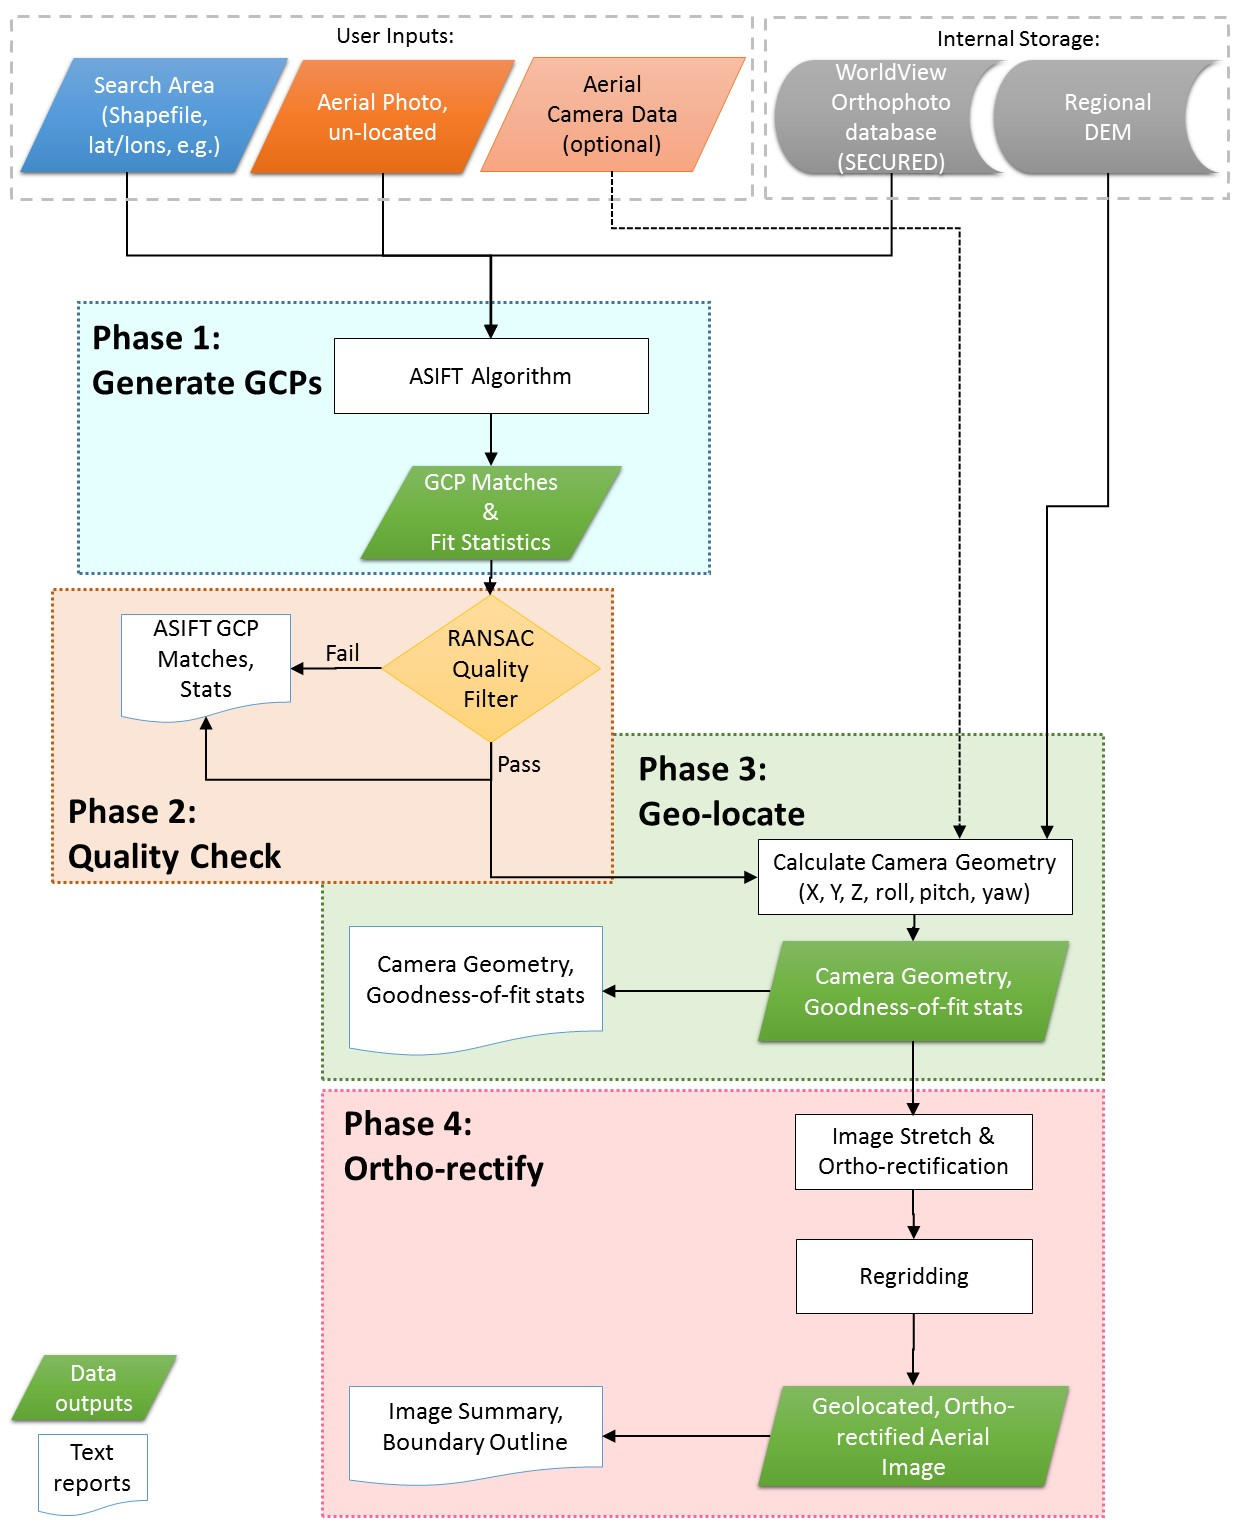
\includegraphics[width=0.8\textwidth]{ASIFTWorkflowDiagram.jpg}
\end{figure}

The main functions of the ASIFT pipeline are generating ground control points (GCPs), 
quality checks (RANSAC), geo-location, ortho-rectification, and  
producing output images.

\section{User Classes and Characteristics}
\iffalse
$<$Identify the various user classes that you anticipate will use this product.  
User classes may be differentiated based on frequency of use, subset of product 
functions used, technical expertise, security or privilege levels, educational 
level, or experience. Describe the pertinent characteristics of each user class.  
Certain requirements may pertain only to certain user classes. Distinguish the 
most important user classes for this product from those who are less important 
to satisfy.$>$
\fi
\begin{itemize}
	\item Community users - Will use a web interface to access the capabilities
	of ICEBERG
	\item Expert users - Will use ICEBERG via command line interface to execute 
	experiments and their use cases.
	\item Developers - Are users that are able to develop additional pipelines 
	and/or change/update existing pipelines. They will be able to use the CLI or 
	directly the resource interfaces.
\end{itemize}

\section{Operating Environment}
\iffalse
$<$Describe the environment in which the software will operate, including the 
hardware platform, operating system and versions, and any other software 
components or applications with which it must peacefully coexist.$>$
\fi
The software's middleware should be able to use Unix-based Operating Systems, such 
as Linux and MacOS. The software has library dependencies as listed in 
Table~\ref{tab:software_dependencies}. $HARD$ dependency to a library is restricted 
to the version shown. $SOFT$ dependency to a library requires as a minimum version 
the one depicted.

The Command Line Interface should be used from a Virtual Machine that is in the 
Cloud and has constant Internet connection.

The Web interface should be hosted on resources with constant operation.

\begin{table}
	\centering
	\begin{tabular}{|c|c|c|c|}
		\hline
		Library & Version & Executable & Type\\\hline
		Python        & 3.5      & All              & $SOFT$\\\hline
		EnTK          & 0.7      & entk\_script     & $SOFT$ \\\hline
		opencv-python & 3.2      & tile\_raster     & $SOFT$ \\\hline
		gdal-python   & 2.2.1    & tile\_raster     & $SOFT$ \\\hline
		USAC          & Any      & All              & $SOFT$ \\\hline
		liblapack-dev & Any      & All              & $SOFT$ \\\hline
		libblas-dev   & Any      & All              & $SOFT$ \\\hline
		libconfig-dev & Any      & All              & $SOFT$ \\\hline
		libconfig++   & Any      & All              & $SOFT$ \\\hline
 		\hline
	\end{tabular}
	\caption{Software Dependencies.\label{tab:software_dependencies}}
\end{table}




\section{Design and Implementation Constraints}
\iffalse
$<$Describe any items or issues that will limit the options available to the 
developers. These might include: corporate or regulatory policies; hardware 
limitations (timing requirements, memory requirements); interfaces to other 
applications; specific technologies, tools, and databases to be used; parallel 
operations; language requirements; communications protocols; security 
considerations; design conventions or programming standards (for example, if the 
customer’s organization will be responsible for maintaining the delivered 
software).$>$
\fi

Access to the VM should be through SSH or GSISSH. The web interface should be under HTTPS 
protocol.

Users should have their image data uploaded to the resources via a secure data 
transfer system, like sftp/scp.

Users should not execute from the login nodes instead the user should execute the job through queue system.

\section{User Documentation}
\iffalse
$<$List the user documentation components (such as user manuals, on-line help, 
and tutorials) that will be delivered along with the software. Identify any 
known user documentation delivery formats or standards.$>$
\fi
Users will be provided on-line documentation and help.  Syntax, options, and error
messages will be displayed via the web or command line interfaces.

\section{Assumptions and Dependencies}
\iffalse
$<$List any assumed factors (as opposed to known facts) that could affect the 
requirements stated in the SRS. These could include third-party or commercial 
components that you plan to use, issues around the development or operating 
environment, or constraints. The project could be affected if these assumptions 
are incorrect, are not shared, or change. Also identify any dependencies the 
project has on external factors, such as software components that you intend to 
reuse from another project, unless they are already documented elsewhere (for 
example, in the vision and scope document or the project plan).$>$

\fi
OpenCV version 3.2.0 and GDAL v2.2.1 is assumed to be compiled and preinstalled on the resources.In order to use SIIM descriptors proposed by OpenCV and inorder to use GEOTIFF imagery. Also Python 2.7 and 3.5 should exist in the resource.
% ----------------------------------------------------------------------------
% Interface Requirements
% ----------------------------------------------------------------------------
\chapter{External Interface Requirements}

\section{User Interfaces}
\iffalse
$<$Describe the logical characteristics of each interface between the software 
product and the users. This may include sample screen images, any GUI standards 
or product family style guides that are to be followed, screen layout 
constraints, standard buttons and functions (e.g., help) that will appear on 
every screen, keyboard shortcuts, error message display standards, and so on.  
Define the software components for which a user interface is needed. Details of 
the user interface design should be documented in a separate user interface 
specification.$>$
\fi

Provide an interface where users can upload an image and get back a table 
with Ground Control Points (GCPs) and ortho-rectified image.

The CLI interface should have the arguments based on table~\ref{tab:cli_interface}

\begin{table}[ht]
	\centering
	\begin{tabular}{|p{2.5cm}|p{2.2cm}|p{1.8cm}|p{4cm}|p{2cm}|}
		\hline
		Argument Name    & Argument Flag(s) & Argument Type & Value & Required/ Optional\\\hline
		Resource         & -r/--resource    & String        & xsede.bridges & Required\\\hline
		Output Directory & -op              & String        & './'    & Optional\\\hline
		Input Directory  & -ip              & String        & /home/iparask/images & Required\\\hline
		\hline
	\end{tabular}
	\caption{Command Line Interface Arguments.\label{tab:cli_interface}}
\end{table}


\section{Hardware Interfaces}
\iffalse
$<$Describe the logical and physical characteristics of each interface between 
the software product and the hardware components of the system. This may include 
the supported device types, the nature of the data and control interactions 
between the software and the hardware, and communication protocols to be 
used.$>$
\fi

The software system requires High Performance Computing (HPC) resources for execution. 
The HPC resources should provide CPU and high amount of Memory(RAM). 
Any XSEDE resource is a good candidate.

\section{Software Interfaces}
$<$Describe the connections between this product and other specific software 
components (name and version), including databases, operating systems, tools, 
libraries, and integrated commercial components. Identify the data items or 
messages coming into the system and going out and describe the purpose of each.  
Describe the services needed and the nature of communications. Refer to 
documents that describe detailed application programming interface protocols.  
Identify data that will be shared across software components. If the data 
sharing mechanism must be implemented in a specific way (for example, use of a 
global data area in a multitasking operating system), specify this as an 
implementation constraint.$>$

\section{Communications Interfaces}
$<$Describe the requirements associated with any communications functions 
required by this product, including e-mail, web browser, network server 
communications protocols, electronic forms, and so on. Define any pertinent 
message formatting. Identify any communication standards that will be used, such 
as FTP or HTTP. Specify any communication security or encryption issues, data 
transfer rates, and synchronization mechanisms.$>$


% ----------------------------------------------------------------------------
% Functional Requirements
% ----------------------------------------------------------------------------
\chapter{System Features}
$<$This template illustrates organizing the functional requirements for the 
product by system features, the major services provided by the product. You may 
prefer to organize this section by use case, mode of operation, user class, 
object class, functional hierarchy, or combinations of these, whatever makes the 
most logical sense for your product.$>$

\section{System Feature 1}
$<$Don’t really say “System Feature 1.” State the feature name in just a few 
words.$>$

\subsection{Description and Priority}
$<$Provide a short description of the feature and indicate whether it is of 
High, Medium, or Low priority. You could also include specific priority 
component ratings, such as benefit, penalty, cost, and risk (each rated on a 
relative scale from a low of 1 to a high of 9).$>$

\subsection{Stimulus/Response Sequences}
$<$List the sequences of user actions and system responses that stimulate the 
behavior defined for this feature. These will correspond to the dialog elements 
associated with use cases.$>$

\subsection{Functional Requirements}
$<$Itemize the detailed functional requirements associated with this feature.  
These are the software capabilities that must be present in order for the user 
to carry out the services provided by the feature, or to execute the use case.  
Include how the product should respond to anticipated error conditions or 
invalid inputs. Requirements should be concise, complete, unambiguous, 
verifiable, and necessary. Use “TBD” as a placeholder to indicate when necessary 
information is not yet available.$>$

$<$Each requirement should be uniquely identified with a sequence number or a 
meaningful tag of some kind.$>$

REQ-1:  REQ-2:

\section{System Feature 2 (and so on)}

% ----------------------------------------------------------------------------
% Nonfunctional Requirements
% ----------------------------------------------------------------------------
\chapter{Other Nonfunctional Requirements}

\section{Performance Requirements}
\iffalse
$<$If there are performance requirements for the product under various 
circumstances, state them here and explain their rationale, to help the 
developers understand the intent and make suitable design choices. Specify the 
timing relationships for real time systems. Make such requirements as specific 
as possible. You may need to state performance requirements for individual 
functional requirements or features.$>$
\fi

There are no performance requirements as of now.

\section{Safety Requirements}
\iffalse
$<$Specify those requirements that are concerned with possible loss, damage, or 
harm that could result from the use of the product. Define any safeguards or 
actions that must be taken, as well as actions that must be prevented. Refer to 
any external policies or regulations that state safety issues that affect the 
product’s design or use. Define any safety certifications that must be 
satisfied.$>$
\fi
All input data are treated as read only. They should not be deleted.

\section{Security Requirements}
\iffalse
$<$Specify any requirements regarding security or privacy issues surrounding use 
of the product or protection of the data used or created by the product. Define 
any user identity authentication requirements. Refer to any external policies or 
regulations containing security issues that affect the product. Define any 
security or privacy certifications that must be satisfied.$>$
\fi
All Digital Globe (WorldView) imagery is proprietary and cannot be released publically. 
Use of imagery must be in accordance with the guidelines and requirements of the Polar 
Geospatial Center and the NGA NextView License. 

\section{Software Quality Attributes}
\iffalse
$<$Specify any additional quality characteristics for the product that will be 
important to either the customers or the developers. Some to consider are: 
adaptability, availability, correctness, flexibility, interoperability, 
maintainability, portability, reliability, reusability, robustness, testability, 
and usability. Write these to be specific, quantitative, and verifiable when 
possible. At the least, clarify the relative preferences for various attributes, 
such as ease of use over ease of learning.$>$\fi

The software should be accompanied with detailed documentation, and examples that demonstrate its usage. In addition, the source code should publicly available through Github.




\iffalse
% ----------------------------------------------------------------------------
% Other Requirements
% ----------------------------------------------------------------------------
\chapter{Other Requirements}
$<$Define any other requirements not covered elsewhere in the SRS. This might 
include database requirements, internationalization requirements, legal 
requirements, reuse objectives for the project, and so on. Add any new sections 
that are pertinent to the project.$>$


% ----------------------------------------------------------------------------
% Appendixes
% ----------------------------------------------------------------------------
\section{Appendix A: Glossary}
%see https://en.wikibooks.org/wiki/LaTeX/Glossary
$<$Define all the terms necessary to properly interpret the SRS, including 
acronyms and abbreviations. You may wish to build a separate glossary that spans 
multiple projects or the entire organization, and just include terms specific to 
a single project in each SRS.$>$

\section{Appendix B: Analysis Models}
$<$Optionally, include any pertinent analysis models, such as data flow 
diagrams, class diagrams, state-transition diagrams, or entity-relationship 
diagrams.$>$

\section{Appendix C: To Be Determined List}
$<$Collect a numbered list of the TBD (to be determined) references that remain 
in the SRS so they can be tracked to closure.$>$
\fi
\end{document}

